\documentclass[11pt,a4paper]{article}

%% Packages
\usepackage[T1]{fontenc}
\usepackage[utf8]{inputenc}
\usepackage{lmodern}
\usepackage[top=2.5cm,bottom=2.5cm,left=2.5cm,right=2.5cm]{geometry}
\usepackage{graphicx}
\usepackage{xcolor}
\usepackage{hyperref}
\usepackage{booktabs}
\usepackage{array}
\usepackage{longtable}
\usepackage{enumitem}
\usepackage{caption}
\usepackage{float}
\usepackage{tikz}
\usetikzlibrary{shapes.geometric,arrows.meta,positioning,fit,backgrounds}
\usepackage{fancyhdr}
\usepackage{titlesec}
\usepackage{parskip}
\usepackage{microtype}
\usepackage{tcolorbox}
\tcbuselibrary{skins,breakable}
\usepackage{setspace}

%% Colours
\definecolor{reportBlue}{RGB}{30,58,138}
\definecolor{lightGray}{RGB}{248,249,250}
\definecolor{midGray}{RGB}{100,116,139}
\definecolor{accentGreen}{RGB}{5,150,105}
\definecolor{accentRed}{RGB}{185,28,28}

%% Hyperref
\hypersetup{colorlinks=true,linkcolor=reportBlue,urlcolor=reportBlue,citecolor=reportBlue,
  pdftitle={MedVault Academic Report},pdfauthor={CMU Africa}}

%% Section headings
\titleformat{\section}{\large\bfseries\color{reportBlue}}{\thesection}{0.8em}{}[\vspace{2pt}\color{reportBlue!40}\rule{\linewidth}{0.5pt}]
\titleformat{\subsection}{\normalsize\bfseries}{\thesubsection}{0.6em}{}
\titleformat{\subsubsection}{\normalsize\itshape}{\thesubsubsection}{0.5em}{}
\titlespacing{\section}{0pt}{14pt}{6pt}
\titlespacing{\subsection}{0pt}{8pt}{3pt}

%% Header and footer
\pagestyle{fancy}\fancyhf{}
\lhead{\small\textit{MedVault: A Security System for Health Facilities in Kigali}}
\rhead{\small\textit{CMU Africa, Spring 2026}}
\cfoot{\thepage}
\renewcommand{\headrulewidth}{0.4pt}

%% Image placeholder
\newcommand{\imgbox}[3]{%
  \begin{figure}[H]
    \centering
    \begin{tikzpicture}
      \fill[lightGray] (0,0) rectangle (\linewidth,#1);
      \draw[midGray,dashed,line width=0.5pt] (0,0) rectangle (\linewidth,#1);
      \node[font=\small\itshape,text=midGray,align=center,text width=0.8\linewidth]
        at (0.5\linewidth,0.5*#1) {#3};
    \end{tikzpicture}
    \caption{#2}
    \label{fig:#2}
  \end{figure}%
}

%% TikZ styles
\tikzset{
  lyr/.style={draw,rounded corners=3pt,minimum width=12cm,minimum height=0.75cm,
              font=\small\bfseries,align=center,text width=11.5cm},
  pstep/.style={draw,rounded corners=3pt,minimum width=10cm,minimum height=0.65cm,
               font=\small,align=center,fill=white},
  arr/.style={-Stealth,thick,midGray},
  sarr/.style={-Stealth,semithick,reportBlue!60},
}

\begin{document}

%% Title page
\begin{titlepage}
  \centering
  \vspace*{3cm}
  {\Large\bfseries\color{reportBlue}
    A Security System for Health Facilities\\[6pt]
    Medical Record Management in Kigali}\par
  \vspace{1.2cm}
  {\normalsize Carnegie Mellon University Africa}\par
  {\normalsize Information Security, Spring 2026}\par
  \vspace{2cm}
  \begin{tcolorbox}[colback=lightGray,colframe=reportBlue!30,
    left=12pt,right=12pt,top=8pt,bottom=8pt,
    fontupper=\small\itshape]
    \textbf{Abstract.}
    This report presents MedVault, a security-focused overlay built for
    healthcare facilities in Kigali, Rwanda. The system addresses a
    documented gap in existing Electronic Medical Record deployments where
    technical safeguards do not meet current data-protection standards.
    Rather than replacing existing infrastructure, MedVault introduces a
    protection layer that enforces strong identity verification, field-level
    encryption, patient-controlled consent, and a tamper-evident audit trail.
    The report covers the system architecture, threat model, protocol design,
    implementation details, and a set of adversarial demonstrations that
    validate each security control.\\[4pt]
    \textit{\textbf{Authors}: Christian,Raissa, Gustave}
  \end{tcolorbox}
  \vfill
  {\small April 2026}
\end{titlepage}

\tableofcontents
\newpage


\section{Introduction}

\begin{tcolorbox}[colback=lightGray,colframe=midGray,
  left=8pt,right=8pt,top=6pt,bottom=6pt,fontupper=\small\itshape]
  This section is reserved for the authors. Write your own contextual
  motivation, problem statement, and contribution summary here.
  Suggested points: EMR adoption in Rwandan hospitals, the regulatory
  context (Law No.\ 058/2021 on personal data protection), the
  paper-digital boundary problem, and how MedVault addresses it.
\end{tcolorbox}

\imgbox{4cm}{fig:intro}{%
  Insert here: a photograph of a hospital reception or ward in Kigali
  showing paper records alongside a computer terminal, or a map of
  Rwanda highlighting healthcare facilities.}

\section{System Architecture}

MedVault is built as a layered security overlay. It sits between client
applications and the data store, enforcing security controls at each
boundary. The design follows a principle of defence in depth: each layer
operates independently, so a failure at one layer does not automatically
compromise the layers below it (chain-log implemented).

\subsection{Layer Structure}
The system is organised into seven layers, shown in Figure~\ref{fig:arch}.
Requests enter at the top and must pass every layer before reaching the
database. The first two layers (Client and TLS Transport) are in the
untrusted zone. Everything from the Replay Guard downward runs inside the
trusted server process.

\begin{figure}[H]
\centering
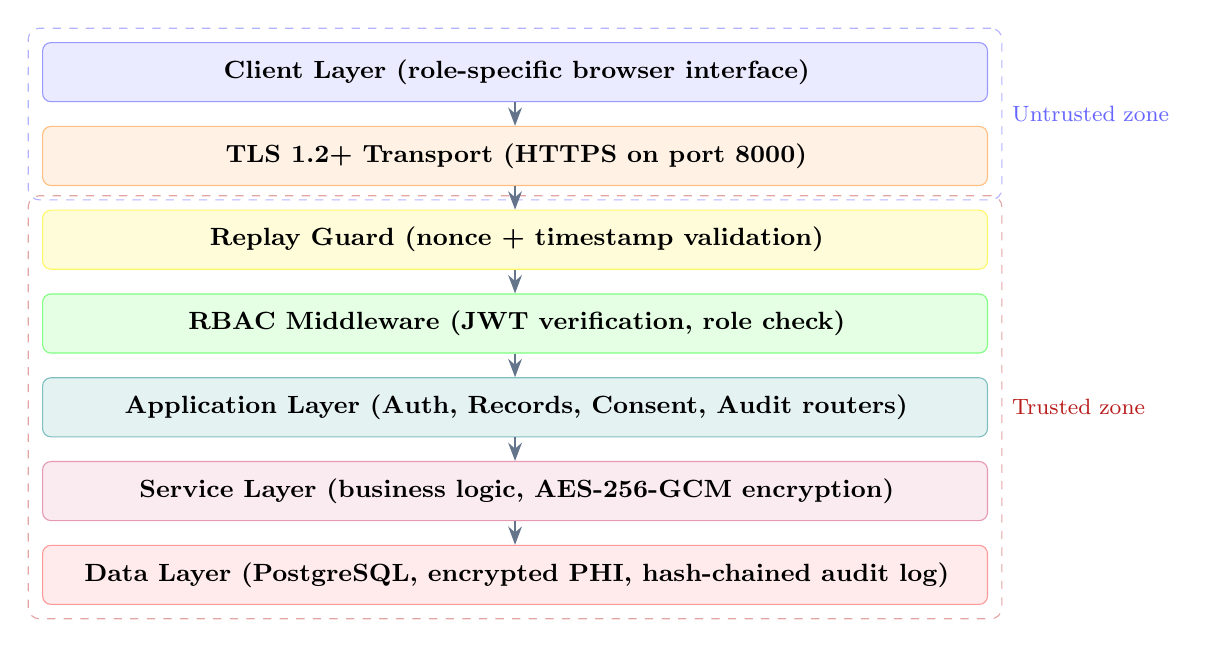
\begin{tikzpicture}[node distance=0.3cm]
  \node[lyr,fill=blue!8,draw=blue!40]    (c)  {Client Layer (role-specific browser interface)};
  \node[lyr,fill=orange!10,draw=orange!50,below=of c]  (t)  {TLS 1.2+ Transport (HTTPS on port 8000)};
  \node[lyr,fill=yellow!15,draw=yellow!60,below=of t]  (rg) {Replay Guard (nonce + timestamp validation)};
  \node[lyr,fill=green!10,draw=green!50,below=of rg]   (rb) {RBAC Middleware (JWT verification, role check)};
  \node[lyr,fill=teal!10,draw=teal!50,below=of rb]     (ap) {Application Layer (Auth, Records, Consent, Audit routers)};
  \node[lyr,fill=purple!8,draw=purple!40,below=of ap]  (sv) {Service Layer (business logic, AES-256-GCM encryption)};
  \node[lyr,fill=red!8,draw=red!40,below=of sv]        (db) {Data Layer (PostgreSQL, encrypted PHI, hash-chained audit log)};
  \foreach \a/\b in {c/t,t/rg,rg/rb,rb/ap,ap/sv,sv/db}
    \draw[arr] (\a.south)--(\b.north);
  \begin{scope}[on background layer]
    \node[draw=blue!30,dashed,rounded corners=4pt,
          fit=(c)(t),inner sep=5pt,
          label={[font=\footnotesize,text=blue!60]right:Untrusted zone}]{};
    \node[draw=accentRed!40,dashed,rounded corners=4pt,
          fit=(rg)(rb)(ap)(sv)(db),inner sep=5pt,
          label={[font=\footnotesize,text=accentRed]right:Trusted zone}]{};
  \end{scope}
\end{tikzpicture}
\caption{Layered architecture with trust boundaries.}
\label{fig:arch}
\end{figure}

\subsection{Security Pipeline}

Every request for medical data passes through a fixed sequence of checks
before any data is returned. The sequence is:

\begin{enumerate}[leftmargin=1.5em,itemsep=2pt]
  \item Verify the JWT signature and expiry.
  \item Confirm the user role permits the requested action.
  \item Check that an active consent grant exists (for doctor access).
  \item Decrypt the record using AES-256-GCM on the server.
  \item Append an audit log entry with the SHA-256 chain hash.
  \item Return the plaintext to the client over the TLS tunnel.
\end{enumerate}

No step can be skipped. Decryption happens entirely on the server; the
client never receives a key or ciphertext.

\subsection{Data Separation}

Encrypted record data (\texttt{encrypted\_data}, \texttt{iv}, \texttt{tag})
is stored in PostgreSQL. The decryption key (\texttt{RECORD\_ENCRYPTION\_KEY})
is loaded from an environment variable at startup and never written to the
database. A full database dump therefore contains only ciphertext.

\imgbox{3.5cm}{fig:dashboard}{%
  Insert here: a screenshot of the MedVault dashboard (doctor or admin
  view) showing the sidebar navigation and a medical record card.
  Capture from the live running system.}


\section{Threat Model}

\subsection{Assets}

The system protects five categories of assets: patient health information
stored in \texttt{medical\_records}; authentication credentials including
password hashes and TOTP secrets; session tokens (access and refresh JWTs);
the encryption keys held in environment configuration; and the audit trail
itself, whose integrity is a prerequisite for non-repudiation.

\subsection{Adversary Classes}

Three adversary classes were considered during design.

\textbf{External attacker.} Has network access and may capture HTTP traffic.
Goals include stealing tokens, replaying captured requests, and reading PHI
in transit.

\textbf{Malicious insider.} Holds valid credentials and may have read access
to the database. Goals include accessing records beyond their role, modifying
the audit trail, and reading encrypted data after a database export.

\textbf{Compromised user.} A legitimate account holder whose credentials have
been stolen or who is subject to social engineering. The main risk is
credential reuse and account takeover.

\subsection{STRIDE Mapping}

Table~\ref{tab:stride} maps each STRIDE category to the primary risk in this
system and the control that addresses it.

\begin{table}[H]
\centering
\small
\setlength{\tabcolsep}{6pt}
\begin{tabular}{p{2.4cm}p{3.5cm}p{5cm}}
\toprule
\textbf{Category} & \textbf{Primary risk} & \textbf{Control} \\
\midrule
Spoofing        & Stolen or weak credentials      & bcrypt hashing, JWT tokens, TOTP MFA \\
Tampering       & Unauthorised record changes     & AES-GCM authentication tag, RBAC \\
Repudiation     & Users deny their actions        & Immutable, hash-chained audit log \\
Disclosure      & PHI exposed in a DB breach      & AES-256-GCM field encryption, TLS \\
Insider threat  & Over-privileged staff access    & Patient-controlled consent, least privilege \\
Provisioning    & Fake or unverified accounts     & Admin-only account creation \\
\bottomrule
\end{tabular}
\caption{STRIDE threat mapping and controls.}
\label{tab:stride}
\end{table}

\section{Protocol Design}

\subsection{Identity and Session Protocol}

Authentication uses a two-step flow. In the first step, the client submits
credentials over HTTPS. The server looks up the account and runs
\texttt{bcrypt.checkpw} against the stored hash. To prevent timing-based
user enumeration, the server always runs a bcrypt check even when the email
does not exist, using a pre-computed dummy hash. If the password is correct
and MFA is not enabled, a full token pair is issued immediately. If MFA is
enabled, a short-lived partial JWT (\texttt{partial=true}, five-minute
expiry) is returned instead.

In the second step, the client submits the partial token together with a
six-digit TOTP code. The server decrypts the stored TOTP secret using
AES-256-GCM, computes the expected code for the current 30-second window
and the adjacent windows (to tolerate clock drift), and compares using
\texttt{hmac.compare\_digest} to prevent timing attacks. On success, a full
access token (15-minute expiry) and a refresh token (7-day expiry, stored
as a SHA-256 hash) are issued.

Refresh tokens are rotated on every use. When a refresh request arrives,
the old token is revoked before the new pair is issued. A stolen refresh
token can therefore only be used once before it becomes invalid.

\subsection{Replay Attack Prevention}

Every state-changing endpoint requires two additional headers:
\texttt{X-Nonce} (a UUID) and \texttt{X-Timestamp} (ISO-8601 UTC). The
Replay Guard middleware checks two conditions before any business logic
runs. First, the timestamp must be within five minutes of the server clock.
Second, the nonce must not appear in the \texttt{nonce\_store} table. If
either check fails, the request is rejected with HTTP 400 before
authentication is attempted. Accepted nonces are stored with a five-minute
TTL, matching the timestamp window, so the table does not grow unboundedly.

\subsection{Transport Security}

All communication runs over TLS 1.2 or higher. The server is started with
the \texttt{--ssl-certfile} and \texttt{--ssl-keyfile} flags passed to
Uvicorn, which wraps every TCP connection in a TLS session before handing
it to FastAPI. The application layer never sees unencrypted bytes.

For the development and demonstration environment, a self-signed certificate
was generated with the following command:

\begin{center}
\small\ttfamily
openssl req -x509 -newkey rsa:4096 -keyout key.pem -out cert.pem \\
\quad -days 365 -nodes \\
\quad -subj \textquotedbl/C=RW/ST=Kigali/O=MedVault/CN=localhost\textquotedbl \\
\quad -addext \textquotedbl subjectAltName=DNS:localhost,IP:127.0.0.1\textquotedbl
\end{center}

This generates a 4096-bit RSA key pair and a self-signed X.509 certificate
valid for one year. The \texttt{-nodes} flag removes the passphrase from
the private key so the server can start without manual intervention. The
\texttt{subjectAltName} extension is required by current browser versions.
The certificate file (\texttt{cert.pem}) is sent to every client during the
TLS handshake. The private key (\texttt{key.pem}) stays on the server.
For production, the certificate paths in \texttt{.env} are updated to point
to a CA-signed certificate. No code change is required.

\subsection{Access Control and Consent}

Role-based access control is enforced by the \texttt{require\_roles()}
dependency applied to every protected endpoint. The dependency decodes the
JWT, reads the \texttt{role} claim, and raises HTTP 403 if the role is not
in the permitted set. Because the role claim is signed inside the JWT, a
user cannot change their role without invalidating the signature.

For doctor access to patient records, role alone is not sufficient. The
records service calls \texttt{\_can\_read()}, which queries
\texttt{consent\_grants} for an active, non-expired grant between the
requesting doctor and the record owner. This check runs inside the service
layer, not at the route level, so it cannot be bypassed by a compromised
route handler. Figure~\ref{fig:pipeline} shows the full sequence.

\begin{figure}[H]
\centering
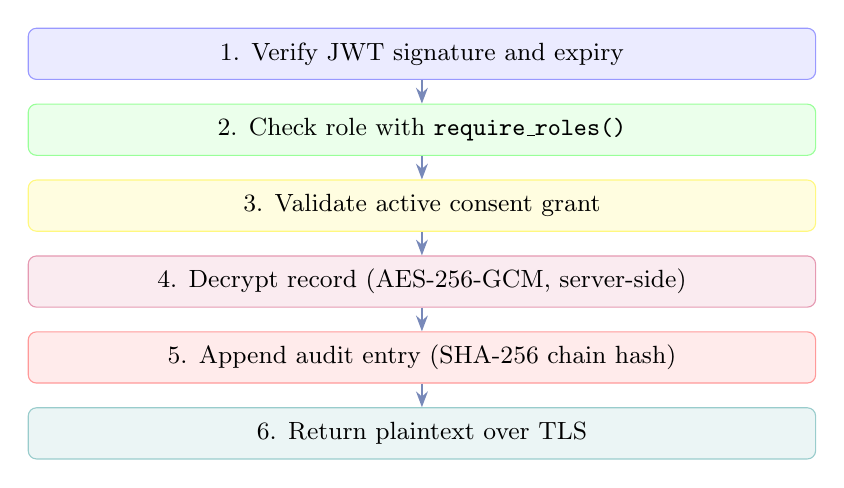
\begin{tikzpicture}[node distance=0.3cm]
  \node[pstep,fill=blue!8,draw=blue!40]    (s1) {1. Verify JWT signature and expiry};
  \node[pstep,fill=green!8,draw=green!40,below=of s1]   (s2) {2. Check role with \texttt{require\_roles()}};
  \node[pstep,fill=yellow!12,draw=yellow!50,below=of s2] (s3) {3. Validate active consent grant};
  \node[pstep,fill=purple!8,draw=purple!40,below=of s3]  (s4) {4. Decrypt record (AES-256-GCM, server-side)};
  \node[pstep,fill=red!8,draw=red!40,below=of s4]        (s5) {5. Append audit entry (SHA-256 chain hash)};
  \node[pstep,fill=teal!8,draw=teal!40,below=of s5]      (s6) {6. Return plaintext over TLS};
  \foreach \a/\b in {s1/s2,s2/s3,s3/s4,s4/s5,s5/s6}
    \draw[sarr] (\a.south)--(\b.north);
\end{tikzpicture}
\caption{Access control pipeline for a medical record read request.}
\label{fig:pipeline}
\end{figure}

\subsection{Encryption Protocol}

Medical records and TOTP secrets are encrypted with AES-256-GCM before
being written to the database. For each encryption operation, a fresh
12-byte initialisation vector is generated using \texttt{os.urandom(12)}.
The ciphertext, IV, and 16-byte authentication tag are stored in separate
columns. On retrieval, the tag is verified before any plaintext is returned.
A mismatch raises \texttt{InvalidTag} and the request fails with HTTP 500.

Two separate 256-bit keys are used: \texttt{RECORD\_ENCRYPTION\_KEY} for
medical records and \texttt{TOTP\_ENCRYPTION\_KEY} for TOTP secrets.
This limits the impact of a key compromise to one data category.
Both keys are loaded from environment variables at startup; the application
refuses to start if either is absent or not exactly 32 bytes.

\subsection{Audit Chain Protocol}

Every sensitive action appends an entry to the audit log. The entry
contains the event type, actor ID, resource ID, resource type, client IP,
and timestamp. Before the entry is written, the service serialises these
fields to a deterministic JSON string (sorted keys, no whitespace) and
computes:

\begin{center}
\small\texttt{chain\_hash = SHA-256(serialised\_entry + previous\_chain\_hash)}
\end{center}

The first entry uses a sentinel of 64 zero characters as the previous hash.
To verify integrity, \texttt{GET /audit/verify} recomputes every hash in
sequence and reports the first entry where the stored hash does not match.
The database application role has \texttt{INSERT} and \texttt{SELECT}
privileges only on \texttt{audit\_log}, so the application process cannot
issue \texttt{UPDATE} or \texttt{DELETE} even if it is compromised.

\section{Implementation}

\subsection{Technology Stack}

The backend is built with Python 3.11 and FastAPI, using SQLAlchemy 2.x
with the asyncpg driver for asynchronous PostgreSQL access. Database schema
changes are managed with Alembic migrations. The cryptography library
provides AES-256-GCM. Password hashing uses bcrypt. JWT operations use
PyJWT. The TOTP module is implemented from scratch using only the Python
standard library (\texttt{hmac}, \texttt{hashlib}, \texttt{struct},
\texttt{time}, \texttt{os}, \texttt{base64}), with no third-party
dependency, to reduce the supply-chain attack surface.

\subsection{Security Components}

Table~\ref{tab:impl} summarises how each security requirement maps to a
concrete implementation component.

\begin{table}[H]
\centering
\small
\setlength{\tabcolsep}{5pt}
\begin{tabular}{p{3cm}p{9.5cm}}
\toprule
\textbf{Component} & \textbf{Implementation} \\
\midrule
Authentication &
  Passwords stored as bcrypt hashes. Login issues a 15-minute HS256 JWT
  with \texttt{role} and \texttt{sub} claims. MFA flow uses a partial JWT
  (\texttt{partial=true}, 5-min expiry) exchanged for a full token pair
  after TOTP verification. Refresh tokens are 32-byte random values stored
  as SHA-256 hashes and rotated on every use. \\
\addlinespace
Access Control &
  \texttt{require\_roles()} FastAPI dependency applied to every protected
  endpoint. Seven roles: Patient, Doctor, Nurse, Lab\_Technician,
  Front\_Desk, Admin, SuperAdmin. Consent check runs inside the service
  layer for doctor access. \\
\addlinespace
Consent &
  Doctor initiates a request; patient approves or rejects. Active grants
  carry an expiry timestamp. Patients can revoke at any time. State
  transitions: PENDING, ACTIVE, REJECTED, REVOKED, EXPIRED. \\
\addlinespace
Encryption &
  AES-256-GCM with a random 12-byte IV per operation. Ciphertext, IV, and
  tag stored in separate columns. Separate keys for records and TOTP
  secrets. Keys loaded from environment variables; startup fails if absent. \\
\addlinespace
Audit Logging &
  SHA-256 hash chain. DB role restricted to INSERT and SELECT on
  \texttt{audit\_log}. Patients can verify their own entries via
  \texttt{GET /audit/verify}. Admins verify the full chain. \\
\addlinespace
Admin Controls &
  SuperAdmin-only account creation. Security alert dashboard at
  \texttt{GET /admin/security-alerts} aggregates LOGIN\_FAILED,
  ACCESS\_DENIED, and replay-blocked events by account and source IP. \\
\addlinespace
Transport &
  TLS 1.2+ via Uvicorn \texttt{--ssl-certfile} and \texttt{--ssl-keyfile}.
  Self-signed certificate for development; CA-signed certificate for
  production, configured through environment variables only. \\
\bottomrule
\end{tabular}
\caption{Security component implementation summary.}
\label{tab:impl}
\end{table}

\subsection{Configuration and Secrets Management}

No secret value appears in source code or version-controlled files.
All secrets are loaded from a \texttt{.env} file at startup. The required
variables are: \texttt{DATABASE\_URL}, \texttt{JWT\_SECRET\_KEY},
\texttt{RECORD\_ENCRYPTION\_KEY}, \texttt{TOTP\_ENCRYPTION\_KEY},
\texttt{TLS\_CERT\_FILE}, and \texttt{TLS\_KEY\_FILE}. The Key Manager
validates each key at startup and terminates the process with a descriptive
error if any variable is missing or if an encryption key is not exactly
32 bytes. A \texttt{.env.example} file with placeholder values is committed
to the repository so that new developers know which variables to set.

\imgbox{3.5cm}{fig:alerts}{%
  Insert here: a screenshot of the security alerts dashboard
  (SuperAdmin view) showing the stat cards for failed logins,
  access denied events, and replay-blocked requests, together
  with the failed-login table. Capture from the live system.}

\subsection{Limitations}

\textbf{TOTP dependency on a smartphone.} TOTP enrollment requires a
compatible authenticator application (Google Authenticator, Authy, or
similar). Users without a smartphone cannot enable MFA, which reduces the
security guarantee for those accounts.

\textbf{Scope of roles.} The seven roles modelled cover the main personnel
categories in a Kigali hospital but are not exhaustive. A full deployment
would integrate with an existing identity directory such as Active Directory
or LDAP.

\textbf{FHIR integration.} The current implementation uses a local
PostgreSQL database. Real-world interoperability with existing EMR systems
(OpenMRS, Bahmni) requires FHIR R4 API adapters, which are outside the
scope of this project.

\textbf{Rate limiting.} Brute-force attempts are recorded in the audit log
and visible to administrators through the security alert dashboard, but
automatic account lockout is not yet implemented.

\section{Attack and Defence Demonstrations}

Eleven attack scenarios were implemented as runnable Python scripts in the
\texttt{attacks/} directory. Each script demonstrates the attack, shows the
system response, and confirms that the defence is active. Table~\ref{tab:attacks}
lists each scenario with its script and the control that blocks it.

\begin{table}[H]
\centering
\small
\setlength{\tabcolsep}{4pt}
\begin{tabular}{p{0.4cm}p{3.8cm}p{4cm}p{4cm}}
\toprule
\textbf{\#} & \textbf{Attack} & \textbf{Script} & \textbf{Defence} \\
\midrule
1  & Replay attack              & \texttt{01\_replay\_attack.py}              & Nonce store rejects duplicate nonce \\
2  & Stale timestamp            & \texttt{02\_stale\_timestamp.py}            & 5-minute timestamp window \\
3  & Privilege escalation       & \texttt{03\_privilege\_escalation.py}       & \texttt{require\_roles()} returns 403 \\
4  & User enumeration           & \texttt{04\_jwt\_forgery.py}                & Identical error for wrong email or password \\
5  & Brute force                & \texttt{05\_user\_enumeration.py}           & LOGIN\_FAILED events in audit log \\
6  & Audit log tampering        & \texttt{07\_audit\_tampering.py}            & SHA-256 hash chain detects modification \\
7  & Unauthorised record access & \texttt{08\_unauthorized\_record\_access.py}& Consent gate in \texttt{\_can\_read()} \\
8  & Cross-patient access       & \texttt{09\_cross\_patient\_access.py}      & Ownership check on \texttt{patient\_id} \\
9  & Draft record leakage       & \texttt{10\_draft\_record\_leakage.py}      & Status filter (\texttt{published} only) \\
10 & AES-GCM ciphertext tamper  & \texttt{11\_aes\_gcm\_tampering.py}         & GCM authentication tag raises InvalidTag \\
11 & Token theft                & (auth flow)                                 & 15-minute expiry, refresh token rotation \\
\bottomrule
\end{tabular}
\caption{Attack scenarios and corresponding defences.}
\label{tab:attacks}
\end{table}

Two scenarios are worth highlighting because they demonstrate properties
that are not obvious from the architecture description alone.

\textbf{AES-GCM ciphertext tampering (scenario 10).} An attacker with
direct database access flips one byte in the \texttt{encrypted\_data}
column using a PostgreSQL \texttt{UPDATE}. When the patient next reads the
record, the server attempts decryption and the GCM tag verification fails.
The \texttt{cryptography} library raises \texttt{InvalidTag} before
returning any plaintext. The same attack against AES-CBC would succeed
because CBC provides no integrity guarantee.

\textbf{Audit log tampering (scenario 6).} An attacker modifies an audit
entry directly in PostgreSQL. The \texttt{GET /audit/verify} endpoint
recomputes the hash chain from the first entry. Because the modified entry
produces a different hash, every subsequent stored hash is also wrong. The
endpoint reports the first broken link, including the entry ID and event
type. Patients can run the same verification on their own entries.

\imgbox{3.5cm}{fig:attacks}{%
  Insert here: terminal screenshots showing two attack demonstrations.
  Left: replay attack returning 400 REPLAY\_NONCE\_SEEN.
  Right: AES-GCM tampering returning 500 after InvalidTag.
  Capture from running the scripts in \texttt{attacks/}.}

\section{Conclusion}

MedVault shows that a meaningful security layer can be added to existing
healthcare infrastructure without replacing it. The system addresses the
five course deliverables: a layered architecture with documented trust
boundaries (Figure~\ref{fig:arch}), a STRIDE threat model
(Table~\ref{tab:stride}), a formally described protocol covering
authentication, encryption, replay prevention, and audit chaining
(Figure~\ref{fig:pipeline}), a working Python prototype with 20 API
endpoints and 12 database tables, and eleven adversarial demonstrations
(Table~\ref{tab:attacks}).

The combination of TLS at the transport layer, JWT and TOTP at
authentication, RBAC and consent at authorisation, AES-256-GCM at storage,
and a hash-chained audit log at accountability means that no single
compromised component exposes the full system. Each layer provides an
independent check that the others do not duplicate.

\vspace{8pt}
\noindent\rule{\linewidth}{0.4pt}
{\small\textit{Tech stack: Python 3.11, FastAPI, PostgreSQL 15,
SQLAlchemy 2, AES-256-GCM, bcrypt, RFC 6238 TOTP, TLS 1.2+.}}

\end{document}
